\documentclass [a4paper, 11pt] {article}

\usepackage [top=1in, bottom=1in, left=0.5in, right=0.5in] {geometry}
\usepackage {graphicx}
\usepackage{natbib}

\begin {document}

\title {CS296: Project Report (Group 13)}
\author {
	Sonone, \textbf {Ashish}\\
	110050022
	\and
	Khandwala, \textbf {Kandarp} S.\\
	110050005
	\and
	Kumar, \textbf {Dhanesh}\\
	110050021
}
\date {}
\maketitle

\section {Creating a Rube-Goldberg Machine Simulation}

A Rube-Goldberg machine is a deliberately over-engineered or overdone machine that performs a very simple task in a very complex fashion, usually including a chain reaction.
We have designed once such contraption (imagined by us in the very first lab), which we (finally) present here. We used Box2D, a 2-dimensional physics simulation engine
(written in C++) to code/implement it. Firstly, in the report, we describe the intention and structure of our machine (and differences from the originally conceived idea) and
then we analyse the code using profiling and timing techniques we have learn so far and critique its performance.

\begin{figure}[htpb]
	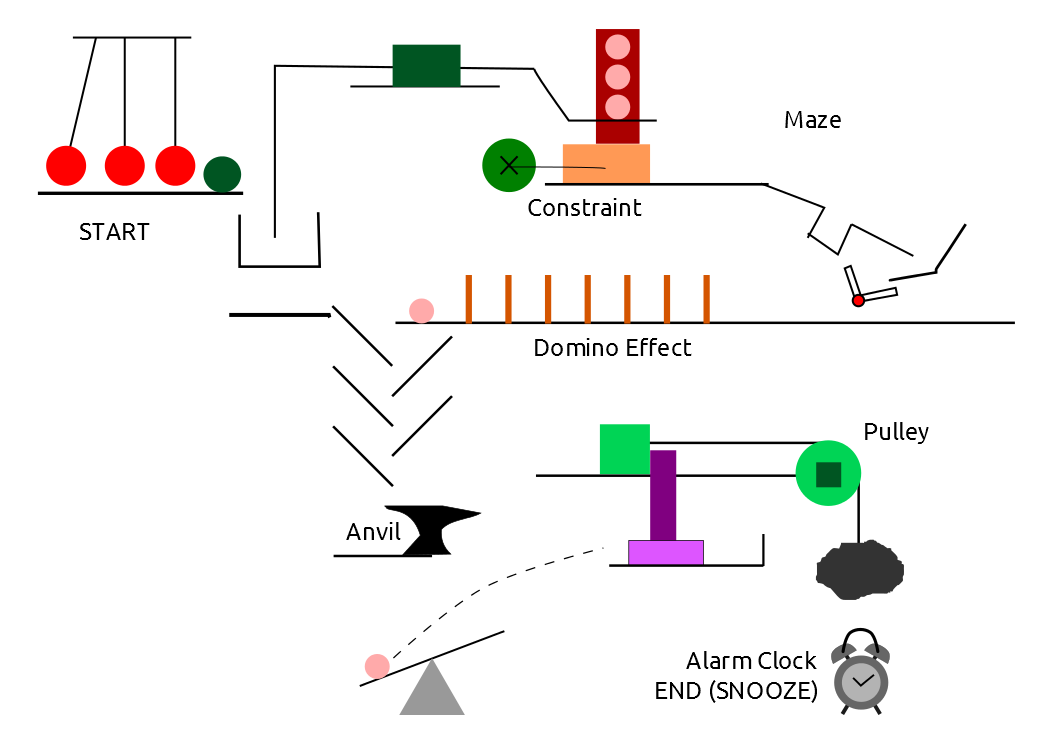
\includegraphics[width=\linewidth]{doc/images/new}
	\caption{Functional Design}
\end{figure}

\section {Design}
The crazy idea we have decided to pursue is: our Rube-Goldberg machine empowers you to crush a buzzing alarm clock, when it disturbs you (damn!) in the morning, right
in the middle of a nice dream, without forgoing the comfort of your bed! Here is how it works: An already moving Newton's Cradle pushes a ball into an open box, which
``unblocks" a stack of 3 balls, one over the other, to be pushed into a maze. The first two balls fill up and align hurdles,with the last ball causing dominos to fall over a ball,
which then reaches a weight, which tipples onto one side of a see-saw. The box on the other side ``flies" like a projectile towards another supporting box, which releases
the pulley to work, finally causing the clock-like object to be snoozed!\\

\noindent{}Some of the interesting pieces in the puzzle are (1) the constrained movement of the block, which pushes the
balls one-by-one as the ``stack" empties itself, (2) the (now simplified) maze and (3) the boulder block waiting to be released, witheld by the blocked box on the other
``side" of the pulley.\\

\noindent{}There arose a couple of differences between the original and finished designs of our Rube-Goldberg machine, namely, replacement of the gear assembly by
a ``string-pulled blocking mechanism" and simplification of the maze \& anvil (since it was becoming tedious). The issue we faced with implementing gears is that we
couldn't figure out how to make performing both translation (not at a fixed position!) and rotational motion simultaneously possible in Box2D, which seems like a limitation
of the gear joint. Maybe, in a future iteration, one could code up a gear from scratch for such purposes!

\begin{figure}[htpb]
	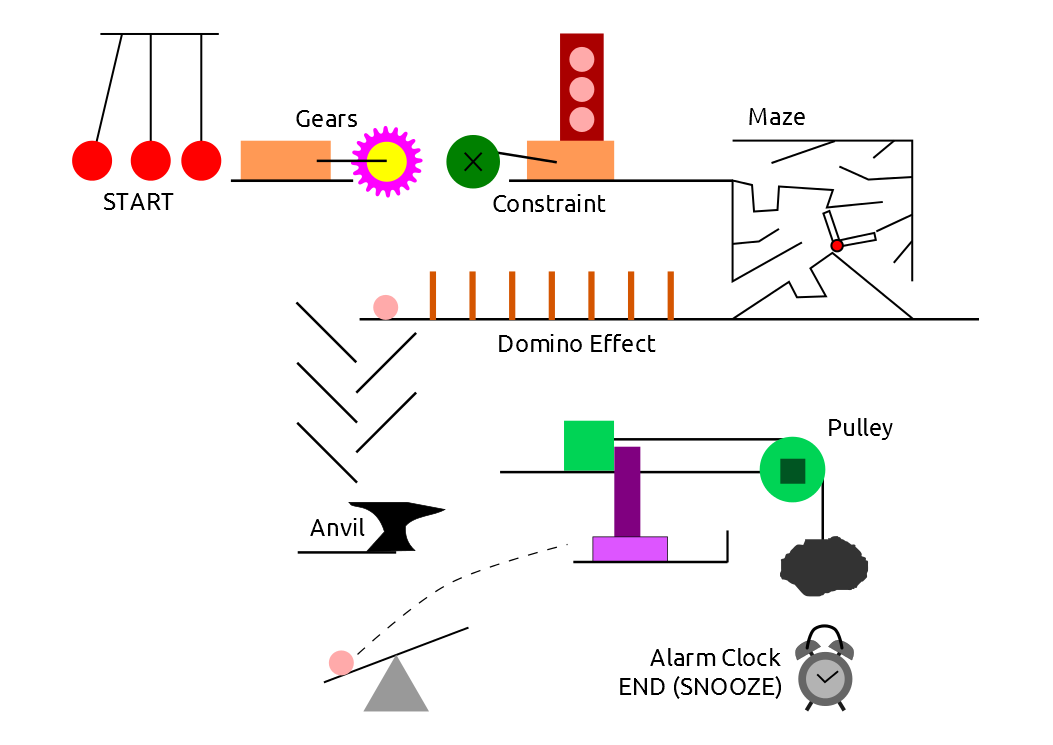
\includegraphics[width=\linewidth]{doc/images/prev}
	\caption{Imagined Design}
\end{figure}

\section {Timing (Plots)}

\begin{figure}[htbp]
  \begin{minipage}{0.5\linewidth}
    \centering
    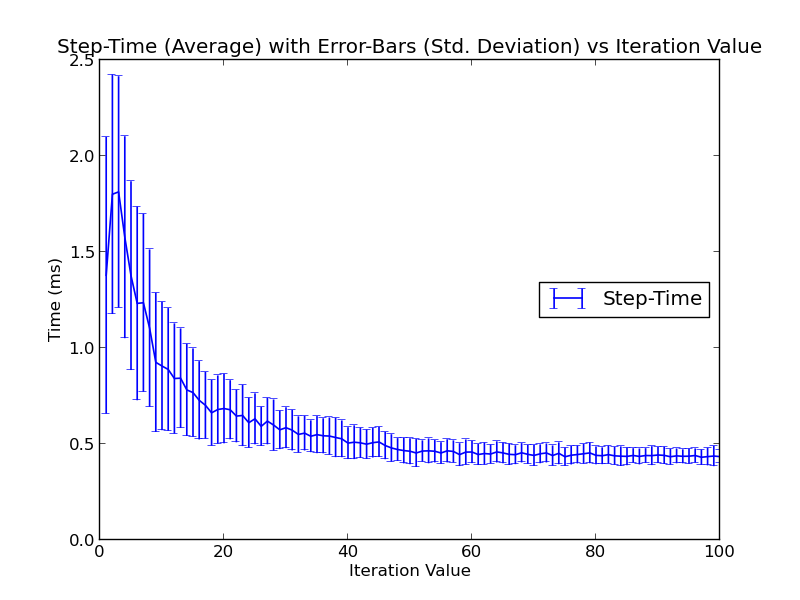
\includegraphics[width=\linewidth]{doc/images/plot05}
    \caption{Step-Time}
  \end{minipage}
  \begin{minipage}{0.5\linewidth}
    \centering
    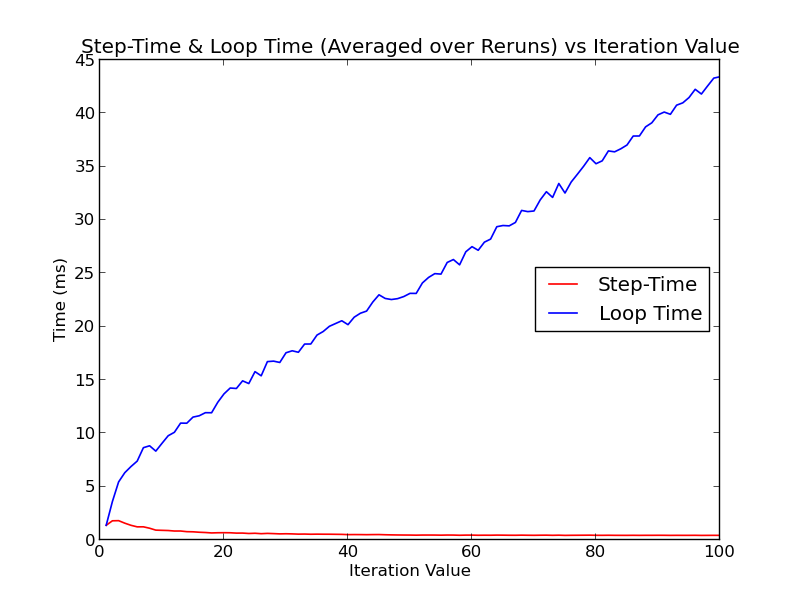
\includegraphics[width=\linewidth]{doc/images/plot01}
    \caption{Loop Time}
  \end{minipage}
\end{figure}

\begin{figure}[htpb]
	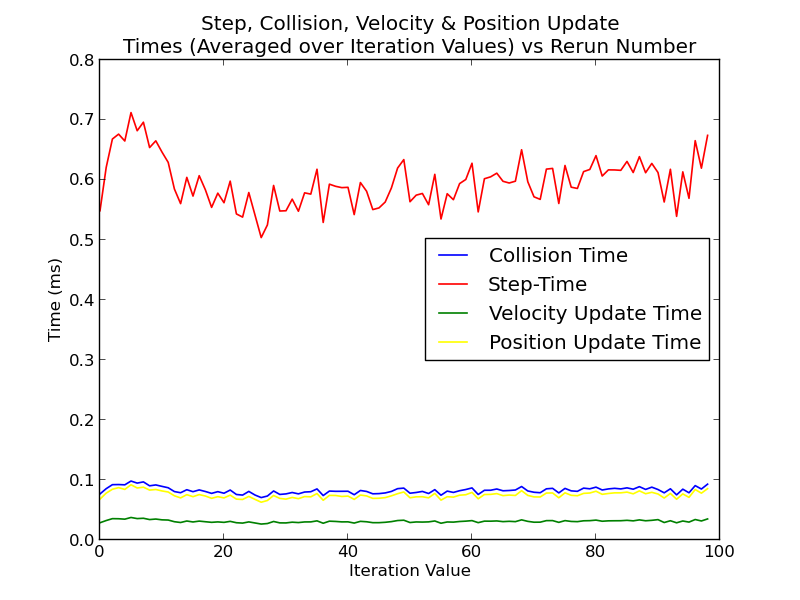
\includegraphics[width=\linewidth]{doc/images/plot04}
	\caption{Various Times vs Rerun Number (Ignore X-Axis Label)}
\end{figure}

\subsection{Step-Time}
\begin{itemize}
	\item Step-time refers to time take to perform one step in the simulation world. It includes the time taken to calculate collision
	time, position and velocity update time apart from other operations.
	\item As number of iterations increases, average step-time per iteration decreases.
	\item Reason 1: It may be that system is slower at start of simulation but as simulation advances, it performs better and makes
	average step-time drop. This may be because a longer process gets priority and is allocated more resources to finish it off quickly.
	\item This trend can be verified when it is run for even higher iteration values like 1000, 5000 or 10000 that average step-time
	diminishes (though only slightly) and conclude that longer the process (number of operations) is lesser the average time for a
	particular operation which eventually approching a lower limit.
	\item Reason 2: It may be because as simulation proceeds calculations in each further step of simulation() are either lesser or
	simpler (so performed faster) and hence average step-time reduces. But this is unlikely that simulation continues to simplify in
	complexity monotonically  for all increasing iteration values.
\end{itemize}

\subsection{Loop Time}
\begin{itemize}
	\item Loop time increases with number of iterations. This is obvious as higher the iterations, more work is to be done, so more time required.
	\item Graph (of loop time vs iterations - see figure) is almost linearly increasing (constant slope).
	\item Again reason is that in our simulation, in the first 100 iterations (upper limit when plotting graphs), same type of work (or computation) is to be done precisely the  pendulum's swinging in Newton's Cradle. Hence, in each step, the same amount of time is taken so the slope is constant.
\end{itemize}

\subsection{Quantities Averaged over Iteration Number vs Rerun Value}
\begin{itemize}
	\item All quantities (Step-time, collision time, velocity time and position time) remain roughly constant with rerun value.\\
	\item This happens as the operating system takes the same amount of time to do the same work for each rerun value in a similar environment.
\end{itemize}

\subsection{Error in Step-Time}
\begin{itemize}
	\item Error in step-time (i.e the standard deviation) diminishes (as clear from the figure) as number of iterations increases, probably because for higher iteration values, the process is more stable (as it runs for a longer time).
\end{itemize}

\section {Performance (Code Profiling)}
We analyzed the two profiles, ``Debug" and ``Release" in order to explore possible inefficiencies in our code. Reiterating what we
learnt in Lab 7, the meaningful difference between the two is that the Debug version is essentially a translation of the code written
manually, with no improvements made by the compiler, while the Release version involves modifications being made in the code
- literally - by the compiler itself. Precisely, the debug version makes no deliberate use of compiler optimizations, both while compiling
the Box2D sources and the object and final binary files, while the Release version - as recommended on
\textit{code.google.com/p/jrfonseca/wiki/Gprof2Dot}, under the heading ``Which options should I pass to GCC when compiling for profiling?"
- uses optimizations covered under the O2 compiler flag (i.e. those which do not involve choosing between any tradeoffs).\\

\noindent{}The call graphs for each of the profiles - for illustrative purposes - are shown below.

\begin{figure}[htbp]
	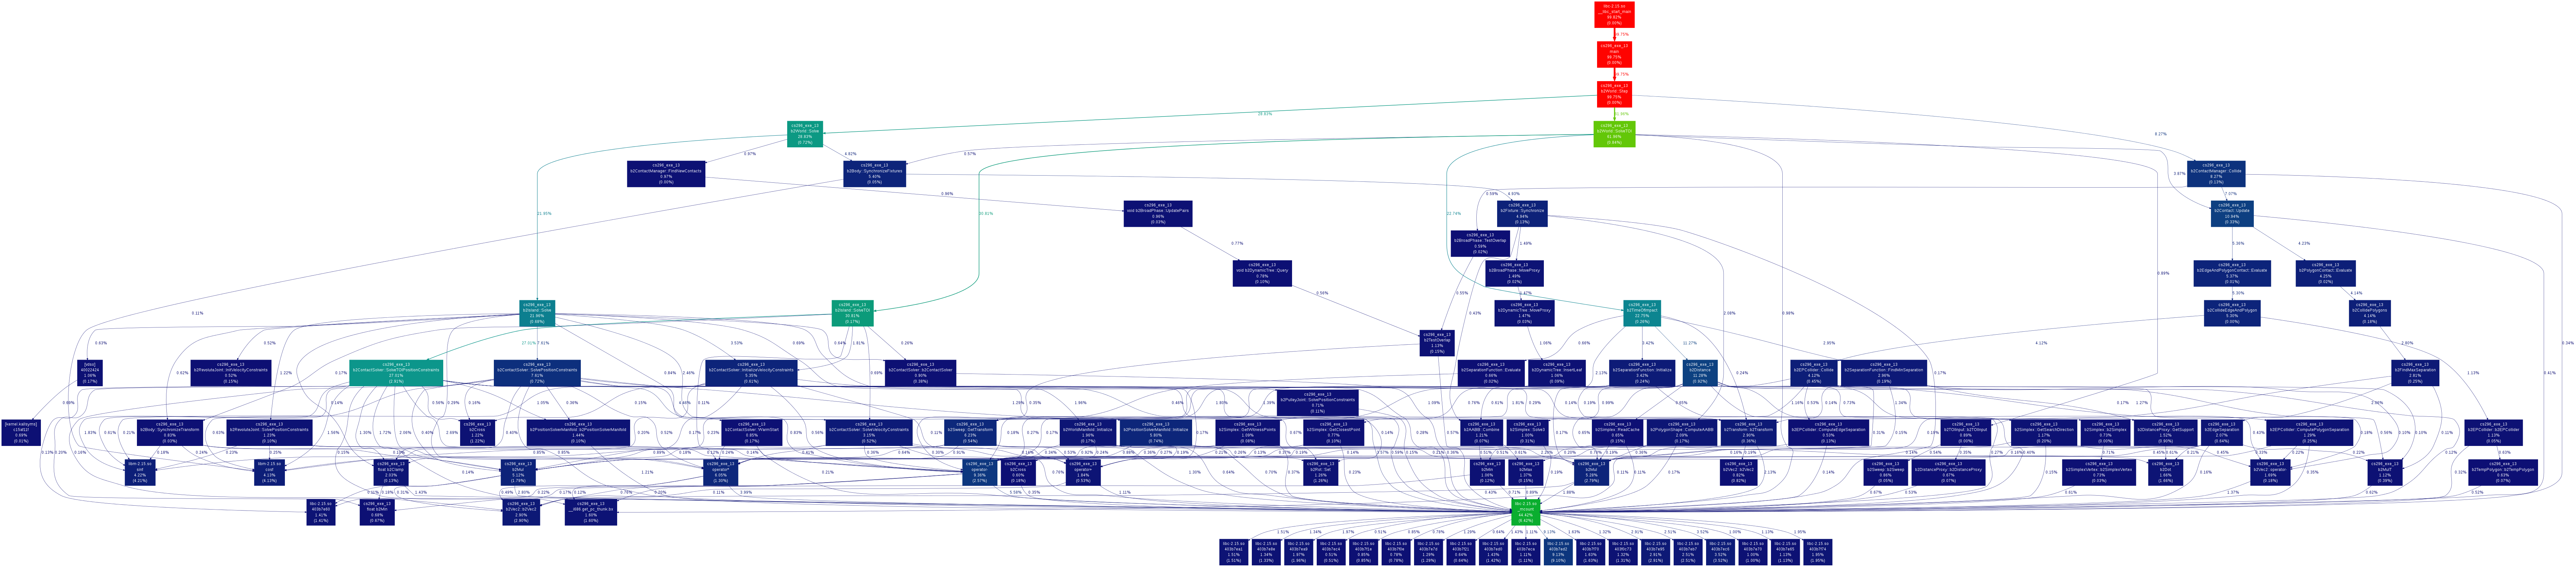
\includegraphics[width=\linewidth]{doc/images/debug10K}
	\caption{Call Graph (code compiled as-is)}
\end{figure}

\noindent{}Differences between the two profiles are also quite prominent (based on the flat profile generated
using gprof), indicating that there is scope to improve the code written, especially some crucial functions.

\begin {itemize}
	\item Firstly, the (inline and similar) functions involving vector operations and the overloaded operators (+, - and *), being called
	a large number of times in the debug version, are not present in the Release version. This seems to happen because these are
	inline functions (w.r.t. operators) or due to the optimizations carried out under the O2 flag (w.r.t. vector manipulating functions).
	\item A notable observation (the opposite of which was evident in Lab 7) is that while the ``bottleneck" functions change - i.e.
	in some cases, those which are more expensive (in terms of time) in the Debug version are often not as expensive in
	the Release version, such as b2ContactSolver::InitializeVelocityConstraints - a side-effect is that some other functions become
	more computationally intensive (such as b2ContactSolver::Solve\\TOIPositionConstraints, b2World::SolveTOI and b2Distance)
	probably since they integrate computations performed by other functions, especially the mathematical (arithmentic and vector)
	operations, called from within their code blocks!
	\item Since b2ContactSolver::SolveTOIPositionConstraints() is one of the non-trivial functions optimized by the compiler in the
	Release version, an interesting observation related to it is that unlike the sample design, which has relatively fewer impacts
	(or instances of contact/collisions between objects), our design entails many such situations occuring, resulting in the
	SolvePositionConstraints() and SolveVelocityConstraints() functions being overshadowed (whereas they were more relevant earlier).
	\item Needless to say, it is obvious (as pointed out in Lab 7 too) that the total running time is drastically reduced in the Release
	version (4.98s from 9.34s). This shows that the O2 flag actually cuts down the total number of computations and hence,
	there do exist redundancies (such as typical pointer evaluations) and more subtle bottleneck-factors in the Box2D implementation,
	which (unfortunately, for now) need a much deeper understanding of the semantics and logic of the code to decrease/eliminate.
	\item Finally, coming to the code written by us, we believe that since it merely involves placing (and choosing the physical
	characteristics of) the various objects provided by Box2D - in other words ``initializing" a ``b2World" - there is not much
	mileage to be gained from optimizing it, though we might be completely mistaken (given our limited knowledge about Box2D)...
\end {itemize}

\begin{figure}[htpb]
	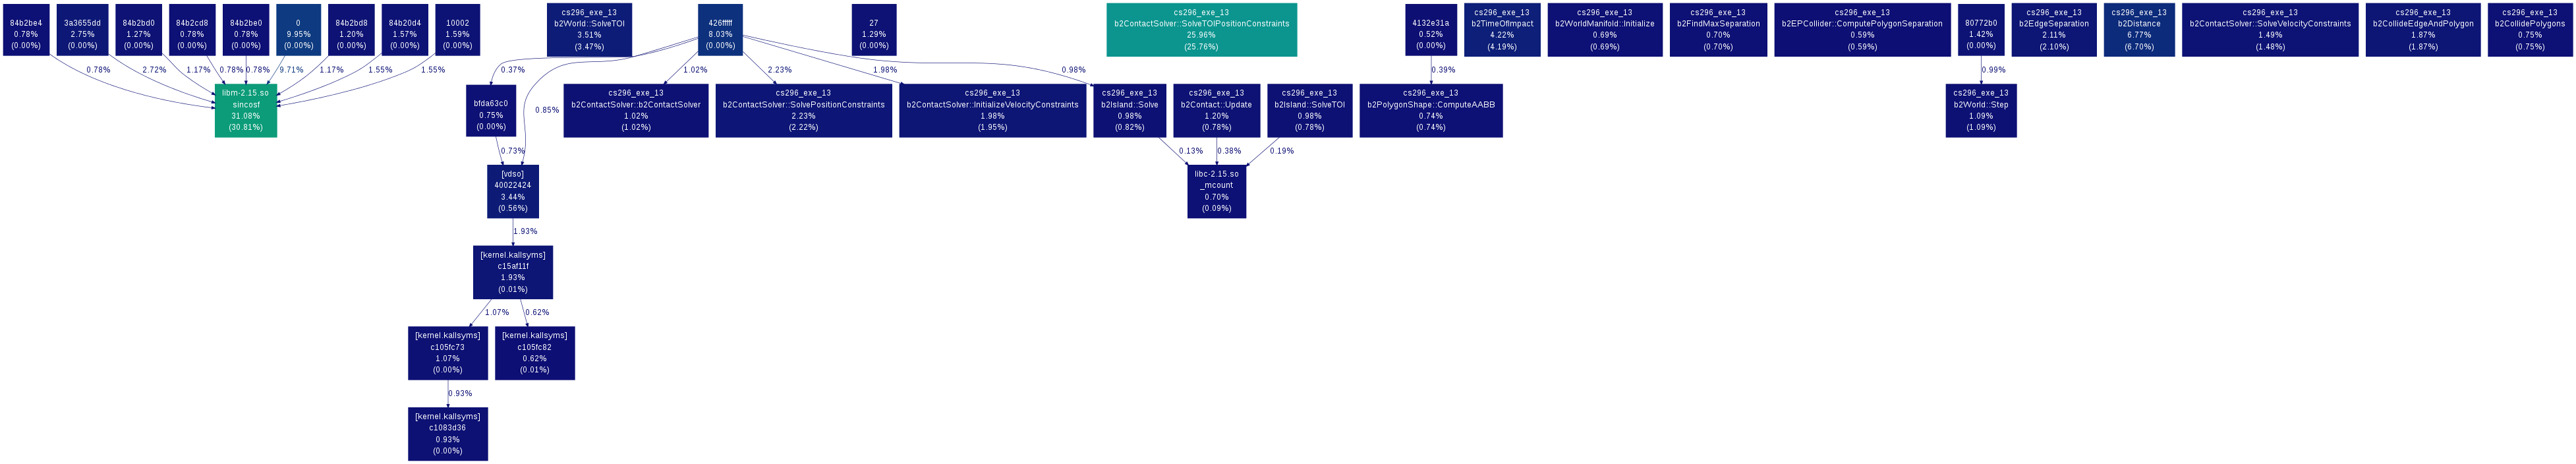
\includegraphics[width=\linewidth]{doc/images/release10K}
	\caption{Call Graph (after automatic optimizations)}
\end{figure}

\section {References}

\begin {enumerate}
	\item http://www.emanueleferonato.com/2009/02/14/box2d-joints-gear-joints\\	
	One example of static (fixed position) gears.
	\item http://www.box2d.org/manual.html\\
	Officially published Box2D documentation.
	\item http://www.iforce2d.net/b2dtut/joints-revolute\\
	Details of the Revolute Joint (Box2D implementation).
	\item http://www.stack.nl/~dimitri/doxygen/manual/docblocks.html\\
	Documentation for Doxygen.
	\item http://www.emanueleferonato.com/2009/01/19/box2d-joints-revolute-joint-building-motors\\
	Implemenation of constrained motion.
\end {enumerate}

\end {document}
